%%%%%%%%%%%%%%%%%%%%%%%============= Functional Requirements =================%%%%%%%%%%%%%%%%%%%%%%%%%
\section{Functional Requirements}
%\begin{itemize}
%	\item Navigation through the use of WiFi Access point data
%	\item Functionality across Android devices
%	\item The application should be developed to function on Google's Play Store.
%	\item Compliance with most recent web accessibility guidelines
%	\item The application should be perceivable, operable, understandable and robust
%	\item Machine vision will be used to detect fiducial markers
%	\item Has to make use of voice recognition technology
%	\item fiducial markers should determine localization and distance from user device
%	\item fiducial markers should notify users of impending obstacles such as bollards
%\end{itemize}

		\subsubsection {REQ1: Navigation}
			Provide navigation functionality.\\ This involves getting a users current position accurately and providing a route to the user's destination.
			
		\subsubsection{REQ2: Usability}
			The system should allow all kinds of users access to helpful navigational information. These users include students, visually and physically impaired students, staff and guests. This involves accessibility and usability issues.
			
		\subsubsection{REQ3: Provide Different Routes}
			Provide different routes based on the user's needs and preferences. This could be for physically or visually impaired users, or by a request for the fastest route taking stairs, ramps, lifts, wheelchair access and obstacles into consideration. %This will require the use of fiducial markers and data capture such as locations of wheelchair ramps/lifts and the machine vision section to detect obstacles.
			
		\subsubsection{REQ4: Mobile deployment}
			The application should be developed so that it may be downloaded from the Google Play Store. %Designs for interfaces should be created with mobile platforms in mind.
		
		\subsubsection{REQ5: User Profiles}
			The system should allow users and administrators login capability and maintain certain information regarding them securely. %This involves the creation and maintenance of a database to store their information. This database should be secure to prevent loss/ theft of data and the system should store only relevant data pertaining to security and law issues. Such issues include the POPI act etc.
			
		\subsubsection{REQ6: User Data Persistence}
			The system should allow users to send information to the system (drop a pin). Examples of such information include location data to allow us to crowdsource dynamic obstacles such as spillages or construction obstacles obscuring traffic or creating potential hazards.%
			
		\subsubsection{REQ7: Accessibility}
			The application should cater for users with access difficulties and impairments. This involves voice recognition activation and compliance with the WCAG.
			Visually impaired users should be informed of impending obstacles to ensure safe navigation to their destination.

		\subsubsection{REQ8: Reliability}
			The application should operate reliably both indoors and outdoors.This is to ensure navigation to all locations correctly on campus.
			
		\subsubsection{REQ9: Integration with campus services}
			The application should integrate with campus services such as the security department or informational systems.
			
		\subsubsection{REQ10: Aesthetics}
			The application appearance should be aesthetically pleasing while conforming to the University of Pretoria's branding styles and colour scheme.

		\subsubsection{REQ11: Machine vision}
			Targeted toward the visually disabled users, the system will be able to read fiducial markers placed around campus. The marker will be read using the user's smartphone camera, thus the user must point the camera in a general forward direction to make use of this feature. Since the user might not always be aware of the exact orientation of his/her device, it is currently under consideration to provide haptic feedback to assist the user in keeping the camera oriented, which will lead to a greater chance of marker detection. The placement of fiducial markers should be placed on walls whenever possible but may be painted on floors where it is not possible. Walls are preferred for two reasons, namely, it is much more cost effective since the marker may be printed on a sheet of paper, secondly, the marker has a greater chance of being detected, with an increase in detection range, when front facing, as opposed to being read at an angle, which is always the case with floor painted markers.

		\subsubsection{REQ12: Landmark notification}
			Targeted toward the visually disabled users and making use of machine vision as specified in the above mentioned functional requirement, the system will notify the user of nearby landmarks that are relevant to the user. Since visually disabled make use of landmarks to a large extent to navigate around campus, thus the intention of landmark notifications is to assist the user with self orientation in order to make the user more effective at moving around campus autonomously. The choice of landmarks and exact nature of the notification will be determined by consulting with Mr Juan Erwee, the technical officer at the disability unit, on a case by case basis.

		\subsubsection{REQ13: Hazard/obstacle notification}
			Targeted toward the visually disabled users and making use of machine vision as specified in the above mentioned functional requirement, the system will notify the user of nearby obstacles and hazards that are relevant to the user. The intention of hazard and obstacle notification is to assist the user in avoiding common hazards and obstacles he/she encounters due to a visual disability. The exact choice of hazard and obstacle as well as the manner in which the information will be conveyed will be determined by consulting with Mr Juan Erwee, the technical officer at the disability unit, on a case by case basis.


%			


%		\subsubsection{REQ6: Personalization}
%			Users should be allowed to save personalized information as well as retrieve it.
%			
%		\subsubsection{REQ7: Maintenance}
%			The system should allow administrators the ability to C.R.U.D(Create,Read,Update,Delete) it.

%
%	\subsection{Possible Nice to Haves?}
%	
%			
%		\subsubsection{REQ11: Weekly goals}
%			Provide weekly goals based on the number of steps or distance traveled by the user.
%			
%		\subsubsection{REQ12: Personalization}
%			Users should be allowed to save personalized information as well as retrieve it.

%			
%		\subsubsection{REQ5: Weekly goals}
%			Provide weekly goals based on the number of steps or distance travelled by the user.
%			
%		\subsubsection{REQ6: Personalization}
%			Users should be allowed to save personalized information as well as retrieve it.%			
%		\subsubsection{REQ5: Weekly goals}
%			Provide weekly goals based on the number of steps or distance travelled by the user.
%			
%		\subsubsection{REQ6: Personalization}
%			Users should be allowed to save personalized information as well as retrieve it.%			
%		\subsubsection{REQ5: Weekly goals}
%			Provide weekly goals based on the number of steps or distance travelled by the user.
%			
%		\subsubsection{REQ6: Personalization}
%			Users should be allowed to save personalized information as well as retrieve it.%			
%		\subsubsection{REQ5: Weekly goals}
%			Provide weekly goals based on the number of steps or distance travelled by the user.
%			
%		\subsubsection{REQ6: Personalization}
%			Users should be allowed to save personalized information as well as retrieve it.%			
%		\subsubsection{REQ5: Weekly goals}
%			Provide weekly goals based on the number of steps or distance travelled by the user.
%			
%		\subsubsection{REQ6: Personalization}
%			Users should be allowed to save personalized information as well as retrieve it.
%		
\newpage
	\subsection{Use Cases}
	
		%%%%%%%%%%%%%%%%%%%%%%======================   UC1    ================%%%%%%%%%%%%%%%%
		\subsubsection{Use Case for REQ1: Navigate user to their desired location}
			\begin{enumerate}
			\renewcommand{\labelenumi}{{\textbf{\arabic{enumi}.}}}
			\item Use Case ID: UC1
			\item Precondition: User is running the NavUP application and enters the navigation module
			\item Postcondition: Client device receives and displays navigational information to destination.
			\item Actor-System interaction model:
				\graphicspath{ {./Diagrams/User/} }
				\begin{figure}[h]
				\caption{Use Case Diagram -  UC1 Navigate user to their desired location}
				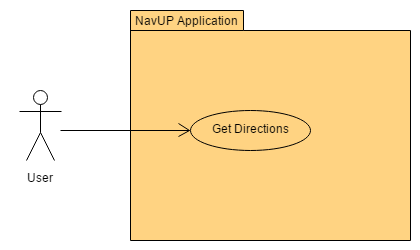
\includegraphics[height = 200px]{GetDesiredLocation.png}
				\end{figure}
			\end{enumerate}

		\begin{table}[htb]
			\centering
			\caption{UC1 -  Navigate user to their desired location}
			\label{my-label}
			\begin{tabular}{|l|l|}
				\hline
				\textbf{Actor: User} &
				\textbf{System: NavUP}
				 \\ \hline  & 0. The NavUP system displays the main window
				\\ \hline
				\begin{tabular}[c]{@{}l@{}}1. The user clicks on the navigation \\ button in the main menu\end{tabular}       &
				\begin{tabular}[c]{@{}l@{}}2. The system displays the navigation page to \\ the user\end{tabular}
				 \\ \hline
				\begin{tabular}[c]{@{}l@{}}3. The user clicks on the Get Directions button\\ on the Navigation page\end{tabular} & 
				\begin{tabular}[c]{@{}l@{}}4. The system prompts the user for their \\ required destination\end{tabular}
				\\ \hline
				5. User enters desired destination & 
				\begin{tabular}[c]{@{}l@{}}6. The system calculates and displays the route\\ and directions to the destination\end{tabular}
				\\ \hline
			\end{tabular}
		\end{table}
				%%%%%%%%%%%%%%%%%%%%%%======================   UC2    ================%%%%%%%%%%%%%%%%
		\newpage
		\subsubsection{Use Case for REQ1: Obtain Current Location}
			\begin{enumerate}
			\renewcommand{\labelenumi}{{\textbf{\arabic{enumi}.}}}
			\item Use Case ID: UC2
			\item Precondition: User is running the NavUP application and requires their location
			\item Postcondition: Client device receives and displays the user's current location data.
			\item Actor-System interaction model:
				\graphicspath{ {./Diagrams/User/} }
				\begin{figure}[h]
				\caption{Use Case Diagram -  UC2  Obtain Current Location}
				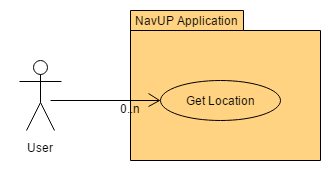
\includegraphics[height = 200px]{ObtainCurrentLocation.png}
				\end{figure}
			\end{enumerate}

		\begin{table}[htb]
			\centering
			\caption{UC2 -  Obtain Current Location}
			\label{my-label}
			\begin{tabular}{|l|l|}
				\hline
				\textbf{Actor: User} &
				\textbf{System: NavUP}
				 \\ \hline  & 0. The NavUP system displays the main window
				\\ \hline
				\begin{tabular}[c]{@{}l@{}}1. The user clicks on the navigation \\ button in the main menu\end{tabular}       &
				\begin{tabular}[c]{@{}l@{}}2. The system displays the navigation page to \\ the user\end{tabular}
				 \\ \hline
				\begin{tabular}[c]{@{}l@{}}3. The user clicks on the Get Location button\\ on the Navigation page\end{tabular} & 
				\begin{tabular}[c]{@{}l@{}}4. The system displays the user's location
				\end{tabular}
				\\ \hline
			\end{tabular}
		\end{table}
		
		
		%%%%%%%%%%%%%%%%%%%%%%======================   UC3    ================%%%%%%%%%%%%%%%%
		\newpage
		\subsubsection{Use Case for REQ1: Search for Location}
			\begin{enumerate}
			\renewcommand{\labelenumi}{{\textbf{\arabic{enumi}.}}}
			\item Use Case ID: UC3
			\item Precondition: User is running the NavUP application and searches for a given location.
			\item Postcondition: Information regarding  the searched location is provided.
			\item Actor-System interaction model:
				\graphicspath{ {./Diagrams/User/} }
				\begin{figure}[h]
				\caption{Use Case Diagram -  UC3  Search for location}
				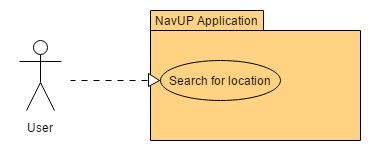
\includegraphics[height = 200px]{SearchForLocation.png}
				\end{figure}
			\end{enumerate}

		\begin{table}[htb]
			\centering
			\caption{UC3 -  Search for location}
			\label{my-label}
			\begin{tabular}{|l|l|}
				\hline
				\textbf{Actor: User} &
				\textbf{System: NavUP}
				 \\ \hline  & 0. The NavUP system displays the main window
				\\ \hline
				\begin{tabular}[c]{@{}l@{}}1. The user clicks on the navigation \\ button in the main menu\end{tabular}       &
				\begin{tabular}[c]{@{}l@{}}2. The system displays the navigation page to \\ the user\end{tabular}
				 \\ \hline
				\begin{tabular}[c]{@{}l@{}}3.  The user clicks on the Search for Location\\ button on the Navigation page\end{tabular} & 
				\begin{tabular}[c]{@{}l@{}}4. The system prompts the user for the \\ location they wish to search\end{tabular}
				\\ \hline
				5. User enters desired location & 
				\begin{tabular}[c]{@{}l@{}}6. The system provides information regarding \\ the searched location\end{tabular}
				\\ \hline
			\end{tabular}
		\end{table}
		
%%%%%%%%%%%%%%%%%%%%%%======================   UC4    ================%%%%%%%%%%%%%%%%
		\newpage
		\subsubsection{Use Case for REQ3: Provide special routes for users with disabilities}
			\begin{enumerate}
			\renewcommand{\labelenumi}{{\textbf{\arabic{enumi}.}}}
			\item Use Case ID: UC4
			\item Precondition: The user is running the application and requires a special route as they have a disability.
			\item Postcondition: Client device recieves and displays information regarding the optimal navigational route for the special needs user.
			\item Actor-System interaction model:
				\graphicspath{ {./Diagrams/User/} }
				\begin{figure}[h]
				\caption{Use Case Diagram - UC4  Provide special routes for users with disabilities}
				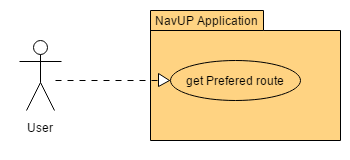
\includegraphics[height = 200px]{getPreferedRoute.png}
				\end{figure}
			\end{enumerate}

		\begin{table}[htb]
			\centering
			\caption{UC4 -  Provide special routes for users with disabilities}
			\label{my-label}
			\begin{tabular}{|l|l|}
				\hline
				\textbf{Actor: User} &
				\textbf{System: NavUP}
				 \\ \hline  & 0. The NavUP system displays the main window
				\\ \hline
				\begin{tabular}[c]{@{}l@{}}1. The user clicks the Routes button on \\the main menu\end{tabular}       &
				\begin{tabular}[c]{@{}l@{}}2. The system prompts the user for \\ a destination\end{tabular}
				\\ \hline
				\begin{tabular}[c]{@{}l@{}}3. The user enters a destination\end{tabular}       &
				\begin{tabular}[c]{@{}l@{}}4. The system prompts the user for \\ the type of route they require\end{tabular}
				\\ \hline
				\begin{tabular}[c]{@{}l@{}}5. The user selects the ''special needs'' option\end{tabular}       &
				\begin{tabular}[c]{@{}l@{}}6. The system displays the route and directions\\ to the destination.\end{tabular}
				\\ \hline
			\end{tabular}
		\end{table}

		%%%%%%%%%%%%%%%%%%%%%%======================   UC5   ================%%%%%%%%%%%%%%%%
		\newpage
		\subsubsection{Use Case for REQ3: Provide the fastest route to a destination}
			\begin{enumerate}
			\renewcommand{\labelenumi}{{\textbf{\arabic{enumi}.}}}
			\item Use Case ID: UC5
			\item Precondition: The user running the application and requires the fastest route from one location to the next.
			\item Postcondition: Client device recieves and displays information regarding the optimal navigational route.
			\item Actor-System interaction model:
				\graphicspath{ {./Diagrams/User/} }
				\begin{figure}[h]
				\caption{Use Case Diagram - UC5  Providethe fastest route to a destination}
				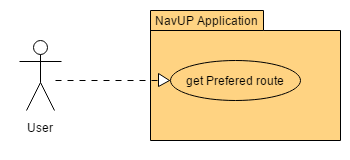
\includegraphics[height = 200px]{getPreferedRoute.png}
		\end{figure}
			\end{enumerate}

		\begin{table}[htb]
			\centering
			\caption{UC5 -  Provide the fastest route to a destination}
			\label{my-label}
			\begin{tabular}{|l|l|}
				\hline
				\textbf{Actor: User} &
				\textbf{System: NavUP}
			 \\ \hline  & 0. The NavUP system displays the main window
				\\ \hline
				\begin{tabular}[c]{@{}l@{}}1. The user clicks the Routes button on \\the main menu\end{tabular}       &
				\begin{tabular}[c]{@{}l@{}}2. The system prompts the user for \\ a destination\end{tabular}
				\\ \hline
				\begin{tabular}[c]{@{}l@{}}3. The user enters a destination\end{tabular}       &
				\begin{tabular}[c]{@{}l@{}}4. The system prompts the user for \\ the type of route they require\end{tabular}
				\\ \hline
				\begin{tabular}[c]{@{}l@{}}5. The user selects the ''fastest path'' option\end{tabular}       &
				\begin{tabular}[c]{@{}l@{}}6. The system displays the route and\\directions to the destination.\end{tabular}
				\\ \hline
			\end{tabular}
		\end{table}
		
		%%%%%%%%%%%%%%%%%%%%%%======================   UC6   ================%%%%%%%%%%%%%%%%
		\newpage
		\subsubsection{Use Case for REQ5: The user logs into the application}
			\begin{enumerate}
			\renewcommand{\labelenumi}{{\textbf{\arabic{enumi}.}}}
			\item Use Case ID: UC6
			\item Precondition: The user wishes to log into the application.
			\item Postcondition: Client device logs the user into the system and displays the user's login page.
			\item Actor-System interaction model:
				\graphicspath{ {./Diagrams/User/} }
				\begin{figure}[h]
				\caption{Use Case Diagram -  UC6 The user logs into the application}
				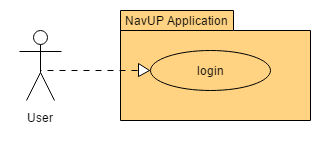
\includegraphics[height = 200px]{Login.png}
				\end{figure}
			\end{enumerate}

		\begin{table}[htb]
			\centering
			\caption{UC6 - The user logs into the application}
			\label{my-label}
			\begin{tabular}{|l|l|}
				\hline
				\textbf{Actor: User} &
				\textbf{System: NavUP}
				 \\ \hline  & 0. The NavUP system displays the main window
				\\ \hline
				\begin{tabular}[c]{@{}l@{}}1. The user clicks the Login button on \\the main menu\end{tabular}       &
				\begin{tabular}[c]{@{}l@{}}2. The system prompts the user to\\ enter the required login details\end{tabular}
				\\ \hline
				\begin{tabular}[c]{@{}l@{}}3. The user enters their login information\end{tabular}       &
				\begin{tabular}[c]{@{}l@{}}4. The system logs the user into the\\ application and displays the user's user page\end{tabular}
				\\ \hline
			\end{tabular}
		\end{table}
		
		%%%%%%%%%%%%%%%%%%%%%%======================   UC7    ================%%%%%%%%%%%%%%%%
		\newpage
		\subsubsection{Use Case for REQ6: Allow users the ability to save a location(drop a pin)}
			\begin{enumerate}
			\renewcommand{\labelenumi}{{\textbf{\arabic{enumi}.}}}
			\item Use Case ID: UC7
			\item Precondition: The user is logged in and wishes to save their location.
			\item Postcondition: Client device displays storage of a location by showing an icon over the specified position.
			\item Actor-System interaction model:
				\graphicspath{ {./Diagrams/User/} }
				\begin{figure}[h]
				\caption{Use Case Diagram - UC7  Allow users the ability to save a location(drop a pin)}
				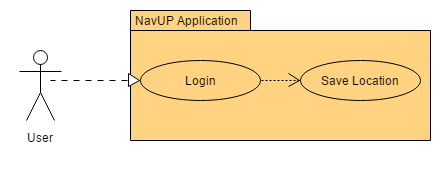
\includegraphics[width = 400px]{SaveL.png}
				\end{figure}
			\end{enumerate}

		\begin{table}[htb]
			\centering
			\caption{UC7 - The user saves a location}
			\label{my-label}
			\begin{tabular}{|l|l|}
				\hline
				\textbf{Actor: User} &
				\textbf{System: NavUP}
				 \\ \hline  & 0. The NavUP system displays the user's page.
				\\ \hline
				\begin{tabular}[c]{@{}l@{}}1. The user clicks the Save Location\\ button\end{tabular}       &
				\begin{tabular}[c]{@{}l@{}}2. The system prompts the user to \\enter a description for the saved location\end{tabular}
				\\ \hline
				\begin{tabular}[c]{@{}l@{}}3. The user enters a description for the\\ saved location and confirms the action\end{tabular}       &
				\begin{tabular}[c]{@{}l@{}}4. The system saves the location and \\displays an icon over the location\end{tabular}
				\\ \hline
			\end{tabular}
		\end{table}

